\chapter{数値的に偏微分方程式を解く}
\label{numerical-partial}
第\ref{analytical-partial}章でも少しお話ししましたが、偏微分方程式は複雑です。数値的に解くとしても統一的な方法はありません。ですので、ここでは基本的な偏微分方程式の形に絞ってその解き方を紹介します。

\section{問題設定}
\label{partial-problem}
ここでは基本的な偏微分方程式として、関数$u(x,y)$について、

\begin{eqnarray}
    A\frac{\partial^2u}{\partial x^2}+2B\frac{\partial^2u}{\partial x\partial y}+C\frac{\partial^2u}{\partial y^2}+D\frac{\partial u}{\partial x}+E\frac{\partial u}{\partial y}+Fu=f(x,y)
    \label{eq:partial-basic}
\end{eqnarray}

\noindent
を考えます。ここで、$A,B,C,D,E,F$は定数、$f(x,y)$は既知の関数だとします。

この形をした偏微分方程式は$AC-B^2$の値で分類でき、それぞれ

\begin{itemize}
    \item $AC-B^2>0$のとき「楕円型」
    \item $AC-B^2=0$のとき「放物型」
    \item $AC-B^2<0$のとき「双曲型」
\end{itemize}

\noindent
と言います。この型が違うと解$u$の挙動が大きく変わります。







\section{差分近似}
\label{partial-difference-calc}
常微分方程式の場合と同様に、2変数関数$u$の差分近似を考えます。まずは$u(x+h,y)$と$u(x-h,y)$についてテイラー展開します。

\begin{eqnarray}
    \label{eq:partial-u-x-1}
    u(x+h,y)&=&u(x,y)+h\frac{\partial}{\partial x}u(x,y)+\frac{h^2}{2!}\frac{\partial^2}{\partial x^2}u(x,y)+\frac{h^3}{3!}\frac{\partial^3}{\partial x^3}u(x,y)+\cdots \\
    \label{eq:partial-u-x-2}
    u(x-h,y)&=&u(x,y)-h\frac{\partial}{\partial x}u(x,y)+\frac{h^2}{2!}\frac{\partial^2}{\partial x^2}u(x,y)-\frac{h^3}{3!}\frac{\partial^3}{\partial x^3}u(x,y)+\cdots
\end{eqnarray}

準備は完了です。まずは$\partial u(x,y)/\partial x$の前進差分近似を求めます。\ref{euler-numerical}節の式を書き直すと、

\begin{eqnarray}
    \frac{\partial}{\partial x}u(x,y)&=&\frac{u(x+h,y)-u(x,y)}{h}+O(h)
\end{eqnarray}

\noindent
となります。これは式\ref{eq:partial-u-x-1}を移項した形をしています。同様にして$y$に関する微分は、

\begin{eqnarray}
    \frac{\partial}{\partial y}u(x,y)&=&\frac{u(x,y+k)-u(x,y)}{k}+O(k)
\end{eqnarray}

\noindent
です。

\if0
後の議論のために中心差分近似も求めておきましょう。式\ref{eq:partial-u-x-1}と式\ref{eq:partial-u-x-2}を辺々引くと、

\begin{eqnarray}
    u(x+h,y)-u(x-h,y)&=&2h\frac{\partial}{\partial x}u(x,y)+O(h^3) \\
    \frac{\partial}{\partial x}u(x,y)&=&\frac{u(x+h,y)-u(x-h,y)}{2h}+O(h^2)
\end{eqnarray}

\noindent
で、局所誤差は$O(h^2)$です。$y$についての微分も同様に、

\begin{eqnarray}
    \frac{\partial}{\partial y}u(x,y)&=&\frac{u(x,y+k)-u(x,y-k)}{2k}+O(k^2)
\end{eqnarray}

\noindent
です。
\fi

また、式\ref{eq:partial-u-x-1}と式\ref{eq:partial-u-x-2}を辺々足すと、

\begin{eqnarray}
    u(x+h,y)+u(x-h,y)&=&2u(x,y)+2\frac{h^2}{2!}\frac{\partial^2}{\partial x^2}u(x,y)+2\frac{h^4}{4!}\frac{\partial^4}{\partial x^4}u(x,y)+\cdots \\
    \frac{\partial^2}{\partial x^2}u(x,y)&=&\frac{u(x+h,y)-2u(x,y)+u(x-h,y)}{h^2}+O(h^2)
\end{eqnarray}

\noindent
二階微分の局所誤差は$O(h^2)$です。$y$についての微分も同様に、

\begin{eqnarray}
    \frac{\partial^2}{\partial y^2}u(x,y)&=&\frac{u(x,y+k)-2u(x,y)+u(x,y-k)}{k^2}+O(k^2)
\end{eqnarray}

最後に$u(x+h,y+k)$をテイラー展開して$\partial^2 u/(\partial x \partial y)$を求めましょう。

\begin{eqnarray}
    u(x+h,y+k)&=&u(x,y)+h\frac{\partial}{\partial x}u(x,y)+k\frac{\partial}{\partial y}u(x,y) \nonumber \\
    &+&\frac{h^2}{2!}\frac{\partial^2}{\partial x^2}u(x,y)+\frac{hk}{2!}2\frac{\partial^2}{\partial x\partial y}u(x,y)+\frac{k^2}{2!}\frac{\partial^2}{\partial y^2}u(x,y)+\cdots \setcounter{equation}{10}
\end{eqnarray}

\noindent
$u(x+h,y+k)$から$u(x+h,y),u(x,y+k)$をそれぞれ引いて、

\begin{eqnarray}
    u(x+h,y+k)-u(x+h,y)-u(x,y+k)=-u(x,y)+hk\frac{\partial^2}{\partial x\partial y}u(x,y)+O(hk(h+k))) \\
    \frac{\partial^2}{\partial x\partial y}u(x,y)=\frac{u(x+h,y+h)-u(x+h,y)-u(x,y+h)+u(x,y)}{hk}+O(hk(h+k)))
\end{eqnarray}

\noindent
とすることで目的の偏導関数が求まりました。局所誤差は$O(hk(h+k)))$です。








\section{陽的差分法}
\label{partial-difference-explicit}
実際に式\ref{eq:partial-basic}に\ref{partial-difference-calc}節での偏導関数を代入し、$u(x,y)=U_{i\ j},\ u(x+h,y)=U_{i+1\ j},\ u(x,y+k)=U_{i\ j+1},\ u(x+h,y+k)=U_{i+1\ j+1}$と置き、係数を適宜置いて、

\begin{eqnarray}
    \label{eq:partial-difference-former}
    2BhkU_{i+1\ j+1}+(Ak^2-2Bhk+Dhk^2)U_{i+1\ j}+(Ch^2-2Bhk+Eh^2k)U_{i\ j+1} \nonumber \\
    +(-2Ak^2+2Bhk-2Ch^2-Dhk^2-Eh^2k+h^2k^2F)U_{i\ j} \nonumber \\
    +Ak^2U_{i-1\ j}+Ch^2U_{i\ j-1}=h^2k^2f(x_i,y_j) \setcounter{equation}{13} \\
    \alpha U_{i+1\ j+1}+\beta U_{i+1\ j}+\gamma U_{i\ j+1}+\delta U_{i\ j}+\epsilon U_{i-1\ j}+\zeta U_{i\ j-1}=\eta f(x_i,y_j)
    \label{eq:partial-difference}
\end{eqnarray}

\noindent
としておきましょう。これを行列を使った式として書いてみます。空白は0です。

\begin{eqnarray}
    \pqty{\begin{array}{ccccc:ccccc:ccccc:c:ccc}
        \delta & \beta & & & & \gamma & \alpha & & & & & & & & & \cdots & & & \\
        \epsilon & \delta & \beta & & & & \gamma & \alpha & & & & & & & & \cdots & & & \\
        & \epsilon & \delta & \beta & & & & \gamma & \alpha & & & & & & & \cdots & & & \\
        & & \ddots & \ddots & \ddots & & & & \ddots & \ddots & & & & & & \cdots & & & \\ %[-2.5pt]
        & & & \epsilon & \delta & & & & & \gamma & & & & & & \cdots & & & \\
        \hdashline
        \zeta & & & & & \delta & \beta & & & & \gamma & \alpha & & & & \cdots & & & \\
        & \zeta & & & & \epsilon & \delta & \beta & & & & \gamma & \alpha & & & \cdots & & & \\
        & & \zeta & & & & \epsilon & \delta & \beta & & & & \gamma & \alpha & & \cdots & & & \\
        & & & \ddots & & & & \ddots & \ddots & \ddots & & & & \ddots & \ddots & \cdots & & & \\ %[-2.5pt]
        & & & & \zeta & & & & \epsilon & \delta & & & & & \gamma & \cdots & & & \\
        \hdashline
        & & & & & \zeta & & & & & \delta & \beta & & & & \cdots & & & \\
        & & & & & & \zeta & & & & \epsilon & \delta & \beta & & & \cdots & & & \\
        & & & & & & & \zeta & & & & \epsilon & \delta & \beta & & \cdots & & & \\
        & & & & & & & & \ddots & & & & \ddots & \ddots & \ddots & \cdots & & & \\
        & & & & & & & & & \zeta & & & & \epsilon & \delta & \cdots & & & \\
        \hdashline
        \vdots & \vdots & \vdots & \vdots & \vdots & \vdots & \vdots & \vdots & \vdots & \vdots & \vdots & \vdots & \vdots & \vdots & \vdots & \ddots & \vdots & \vdots & \vdots \\
        \hdashline
        & & & & & & & & & & & & & & & \cdots & \delta & & \\
        & & & & & & & & & & & & & & & \cdots & & \ddots & \\
        & & & & & & & & & & & & & & & \cdots & & & \delta \\
    \end{array}} \nonumber \\
    \pqty{\begin{array}{c}
        U_{1\ 1} \\
        U_{2\ 1} \\
        U_{3\ 1} \\
        \vdots \\
        U_{N-1\ 1} \\
        \hdashline
        U_{1\ 2} \\
        U_{2\ 2} \\
        U_{3\ 2} \\
        \vdots \\
        U_{N-1\ 2} \\
        \hdashline
        U_{1\ 3} \\
        U_{2\ 3} \\
        U_{3\ 3} \\
        \vdots \\
        U_{N-1\ 3} \\
        \hdashline
        \vdots \\
        \hdashline
        U_{1\ N-1} \\
        \vdots \\
        U_{N-1\ N-1}
    \end{array}}
    =\pqty{\begin{array}{c}
        \eta f(x_1,y_1)-\epsilon U_{0\ 1}-\zeta U_{1\ 0} \\
        \eta f(x_2,y_1)-\zeta U_{2\ 0} \\
        \eta f(x_3,y_1)-\zeta U_{3\ 0} \\
        \vdots \\
        \eta f(x_{N-1},y_1)-\alpha U_{N\ 2}-\beta U_{N\ 1}-\zeta U_{N-1\ 0} \\
        \hdashline
        \eta f(x_1,y_2)-\epsilon U_{0\ 2} \\
        \eta f(x_2,y_2) \\
        \eta f(x_3,y_2) \\
        \vdots \\
        \eta f(x_{N-1},y_2)-\alpha U_{N\ 3}-\beta U_{N\ 2} \\
        \hdashline
        \eta f(x_1,y_3)-\epsilon U_{0\ 3} \\
        \eta f(x_2,y_3) \\
        \eta f(x_3,y_3) \\
        \vdots \\
        \eta f(x_{N-1},y_3)-\alpha U_{N\ 4}-\beta U_{N\ 3} \\
        \hdashline
        \vdots \\
        \hdashline
        \eta f(x_1,y_{N-1})-\alpha U_{N\ N}-\gamma U_{N-1\ N} \\
        \vdots \\
        \eta f(x_{N-1},y_{N-1})-\alpha U_{N\ N}-\beta U_{N\ N-1}-\gamma U_{N-1\ N}
    \end{array}}
    \label{eq:numerical-partial-all}
    \setcounter{equation}{15}
\end{eqnarray}

ここで、境界条件として$(U_{0\ 0},U_{0\ 1}\cdots U_{0\ N})$、$(U_{1\ 0},U_{2\ 0}\cdots U_{N\ 0})$、$(U_{N\ 1},U_{N\ 2}\cdots U_{N\ N})$、\\\noindent$(U_{1\ N},U_{2\ N}\cdots U_{N-1\ N})$がわかっているとします。

陽的差分法の場合、$\alpha=0$である必要があります(そうでない場合は\ref{partial-difference-implicit}節でお話しします)。これは一見、巨大な連立一次方程式です。しかし、式\ref{eq:partial-difference}を見ると未知の量が$U_{i+1\ j}$、$X$を任意として既知の量が$U_{i\ X}$です。未知の量が一つしかないため、連立一次方程式ではなく個々の一次方程式を$i$が小さいものから順番に解くだけで済みます。

では実際に後の議論のため、拡散方程式

\begin{eqnarray}
    \frac{\partial u}{\partial t}=\frac{\partial^2u}{\partial x^2}
\end{eqnarray}

\noindent
を陽的差分法で解いてみましょう。問題にする領域は$0<x<1$かつ$0<t$とします。初期条件

\begin{eqnarray}
    t=0\mbox{で}u=\phi(x)
\end{eqnarray}

\noindent
および、境界条件

\begin{eqnarray}
    x=0,1\mbox{で}u=0
\end{eqnarray}

\noindent
が与えられているとします。

式\ref{eq:partial-basic}において、拡散方程式は$C=1, D=-1$($t$には$x,h$、$x$には$y,k$を対応させます)とし、残りを0とした方程式と見ることができます。よって、これは式\ref{eq:partial-difference}において、$\beta=-hk^2,\gamma=h^2,\delta=-2h^2+hk^2,\zeta=h^2$とし、残りを0とした方程式です。式\ref{eq:partial-difference}を書き直すと、

\begin{eqnarray}
    -hk^2U_{i+1\ j}+h^2U_{i\ j+1}+(-2h^2+hk^2)U_{i\ j}+h^2U_{i\ j-1}=0
\end{eqnarray}

\noindent
となります。これを整理して、

\begin{eqnarray}
    U_{i+1\ j}-U_{i\ j}=\frac{h}{k^2}(U_{i\ j+1}-2U_{i\ j}+U_{i\ j-1}) \\
    U_{i+1\ j}=\frac{h}{k^2}U_{i\ j+1}+\pqty{1-2\frac{h}{k^2}}U_{i\ j}+\frac{h}{k^2}U_{i\ j-1}
    \label{eq:diffusion}
\end{eqnarray}

\noindent
として、未知の$U_{i+1\ j}$を既知の$U_{i,X}$($X$は任意)のみで表せました。初期条件$U_{0\ X}$、および境界条件$U_{X\ 0},U_{X\ N}$($kN=1$)は既知なので、これで初期条件と境界条件を使ってこの偏微分方程式が数値的に解けます。

陽的差分法は$h$と$k$の条件によってはどれだけ$h$や$k$を小さくしても、解が厳密解から大きく外れることがあります。実際に陽的差分法で一つ偏微分方程式を解いてみて、この「解の安定性」を議論しましょう。











\subsection{フォン・ノイマンの安定性解析}
\label{explicit-stability}
陽的差分法で解いた拡散方程式の解の安定性を確かめましょう。ここでは、「フォン・ノイマンの安定性解析」を用います。まず関数$U(t_i,x)$が$x$の区間$(0,1)$でフーリエ級数展開可能だとしましょう\footnote{偏微分方程式を扱うときは大抵フーリエ級数展開可能ですが、もし不可能な場合には式\ref{eq:numerical-partial-all}の固有値の収束性を議論します。}。

関数$U_{i\ j}$を、$\mathrm{i}$を虚数単位、$C_{l\ i}$を未知定数として、

\begin{eqnarray}
    U_{i\ j}=\sum_{l=-\infty}^\infty C_{l\ i}e^{\mathrm{i}2\pi lx_j}
\end{eqnarray}

\noindent
と書くことにします。これを\ref{eq:diffusion}に代入し、$0<x_j<1$なので$x_j=jk$と置きます。すると$\sum$を外すことができ、それぞれの$l$について、

\begin{eqnarray}
    C_{l\ i+1}e^{\mathrm{i}2\pi ljk}&=&\frac{h}{k^2}C_{l\ i}e^{\mathrm{i}2\pi l(j+1)k}+\pqty{1-2\frac{h}{k^2}}C_{l\ i}e^{\mathrm{i}2\pi ljk}+\frac{h}{k^2}C_{l\ i}e^{\mathrm{i}2\pi l(j-1)k} \\
    C_{l\ i+1}&=&\pqty{\frac{h}{k^2}e^{\mathrm{i}2\pi lk}+1-2\frac{h}{k^2}+\frac{h}{k^2}e^{-\mathrm{i}2\pi lk}}C_{l\ i}
\end{eqnarray}


オイラーの公式$e^{\mathrm{i}\theta}=\mathrm{i}\sin\theta+\cos\theta$を使うと、

\begin{eqnarray}
    C_{l\ i+1}&=&\pqty{1-2\frac{h}{k^2}+2\frac{h}{k^2}\cos(2\pi lk)}C_{l\ i} \\
    C_{l\ i+1}&=&\pqty{1-4\frac{h}{k^2}\sin^2(\pi lk)}C_{l\ i}
    \label{eq:difference-stability}
\end{eqnarray}

\noindent
となり、すっきりしました。

ここで、今後の理解に必要な「ラックスの同等定理」を紹介します。ラックスの同等定理は、偏微分方程式の解の収束性を議論するときに使われます。まさに今必要な定理ですね。式\ref{eq:difference-stability}を一般化した

\begin{eqnarray}
    C_{l\ i+1}=gC_{l\ i}
    \label{eq:difference-stability-general}
\end{eqnarray}

\noindent
という式において、どんな$C_{l\ i}$の$i$乗についても

\begin{eqnarray}
    |C_{l\ i}^i|<B
\end{eqnarray}

\noindent
を満たす正の定数$B$が必ず存在するなら、微分方程式を数値的に解いた解は$(h,k)\rightarrow(0,0)$で厳密解に収束します。このことを「解が安定する」と言います。

式\ref{eq:difference-stability-general}は等比数列を表す漸化式と見ることができます。よって、解が安定する条件は、

\begin{eqnarray}
    -1\leq g\leq1
\end{eqnarray}

\noindent
です。

さて、元の議論に戻りましょう。ラックスの同等定理から、式\ref{eq:difference-stability}において、

\begin{eqnarray}
    -1\leq1-4\frac{h}{k^2}\sin^2(\pi lk)\leq1
\end{eqnarray}

\noindent
なら解が安定します。これを変形して、

\begin{eqnarray}
    0\leq\frac{h}{k^2}\sin^2(\pi lk)\leq\frac{1}{2}
\end{eqnarray}

\noindent
を得ます。任意の$\theta$において$0\leq\sin^2\theta\leq1$で、$0<h,k$なので、結局$h$と$k$が満たすべき条件は、

\begin{eqnarray}
    \frac{h}{k^2}\leq\frac{1}{2}
\end{eqnarray}

\noindent
が、解が安定する条件です。

実際に$h=0.004,k=0.1$のとき($h/k^2=0.4$)で計算した結果を図\ref{fig:stability-1}に、$h=0.0052,k=0.1$のとき($h/k^2=0.52$)で計算した結果を図\ref{fig:stability-2}に示します。

\begin{figure}[ht!]
 \begin{minipage}{0.45\hsize}
  \begin{center}
   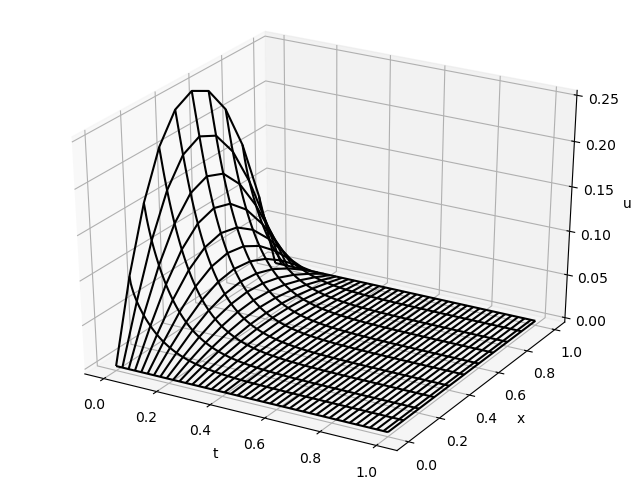
\includegraphics[width=7cm]{img/5-stability1.png}
  \end{center}
  \caption{安定している解}
  \label{fig:stability-1}
 \end{minipage}
 \begin{minipage}{0.5\hsize}
  \begin{center}
   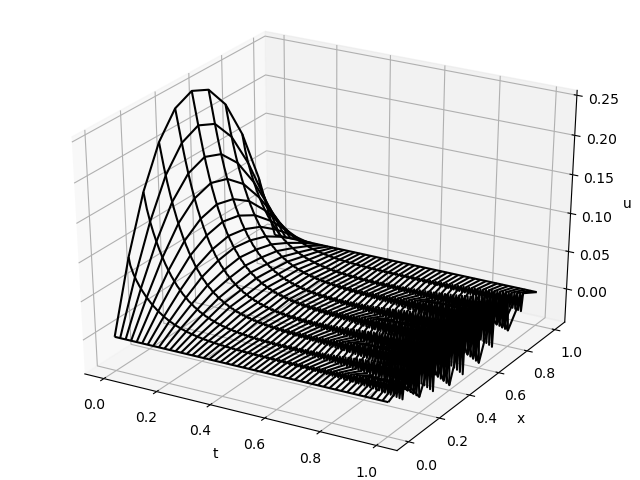
\includegraphics[width=7cm]{img/5-stability2.png}
  \end{center}
  \caption{安定していない解}
  \label{fig:stability-2}
 \end{minipage}
\end{figure}









\section{陰的差分法}
\label{partial-difference-implicit}
陽的差分法では解が安定するために$h$と$k$に条件がありました。それに対し陰的差分法では条件が緩くなったり、完全になくなってしまったりします。

\ref{partial-difference-explicit}節で「陽的差分法で解くには式\ref{eq:partial-difference}の$\alpha$が0である必要がある」と書きました。$\alpha\neq0$のときは$U_{i+1\ j+1}$と$U_{i+1\ j}$の2つの数が未知として1つの式に出てしまうからです。この場合は連立一次方程式\ref{eq:numerical-partial-all}を解くことになります。この行列は疎なので、\ref{gauss-seidel}節で紹介したガウス・ザイデル法などを使って解くことができます。

また、式\ref{eq:partial-difference}で$\alpha=0$である場合にも、差分近似を別のものにしたり、適当に$i$と$j$をずらしたりすることで陰解法に帰着できる場合があります。実際に拡散方程式を解いて確認してみましょう。

陰的差分法で拡散方程式を解くには$\partial u(x,y)/\partial x$および$\partial u(x,y)/\partial y$を後退差分近似に置き換えます。

\begin{eqnarray}
    \frac{\partial}{\partial x}u(x,y)=\frac{u(x,y)-u(x-h,y)}{h}+O(h) \\
    \frac{\partial}{\partial y}u(x,y)=\frac{u(x,y)-u(x,y-k)}{h}+O(k)
\end{eqnarray}

これと\ref{partial-difference-calc}節で紹介した差分近似を代入して、拡散方程式は

\begin{eqnarray}
    \frac{u(t,x)-u(t-h,x)}{h}&=&\frac{u(t,x+k)-2u(t,x)+u(t,x-k)}{k^2} \\
    \frac{U_{i\ j}-U_{i-1\ j}}{h}&=&\frac{U_{i\ j+1}-2U_{i\ j}+U_{i\ j-1}}{k^2}
\end{eqnarray}

\noindent
となります。ここで、$i=i+1$と置換しましょう。

\begin{eqnarray}
    \frac{U_{i+1\ j}-U_{i\ j}}{h}=\frac{U_{i+1\ j+1}-2U_{i+1\ j}+U_{i+1\ j-1}}{k^2} \\
    -\frac{h}{k^2}U_{i+1\ j+1}+\pqty{1+2\frac{h}{k^2}}U_{i+1\ j}-\frac{h}{k^2}U_{i+1\ j-1}=U_{i\ j}
    \label{eq:implicit-diffusion}
\end{eqnarray}

$X$を任意として、左辺にある$U_{i+1\ X}$が未知、右辺の$U_{i\ j}$が未知であるとすると、これは連立一次方程式を解く必要がありそうです。解を求めるのに連立一次方程式を解く必要がある差分法を「陰的差分法」と言います。実際にこれを、陽的差分法で安定しなかったパラメータ$h=0.0052,k=0.1$($h/k^2=0.52$)で解いた結果は図\ref{fig:stability-3}です。また、$h=k=0.1$($h/k^2=10$)でも実験し、図\ref{fig:stability-4}に掲載しました。

\begin{figure}[ht!]
 \begin{minipage}{0.45\hsize}
  \begin{center}
   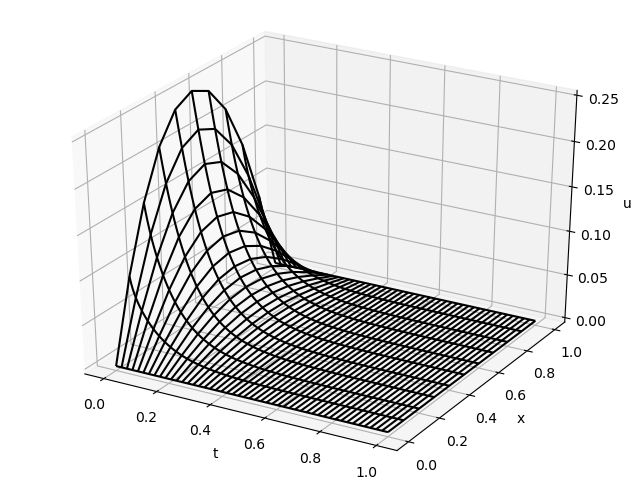
\includegraphics[width=7cm]{img/5-stability3.png}
  \end{center}
  \caption{$h=0.0052,k=0.1$}
  \label{fig:stability-3}
 \end{minipage}
 \begin{minipage}{0.5\hsize}
  \begin{center}
   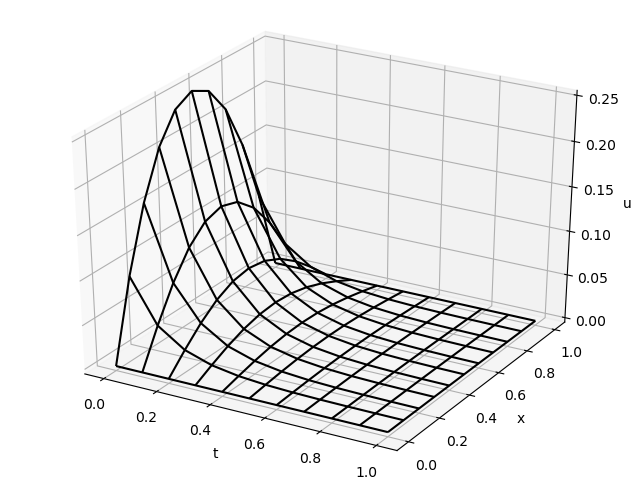
\includegraphics[width=7cm]{img/5-stability4.png}
  \end{center}
  \caption{$h=k=0.1$}
  \label{fig:stability-4}
 \end{minipage}
\end{figure}








\subsection{フォン・ノイマンの安定性解析}
\label{implicit-stability}
では安定性解析を行いましょう。結論から言えば、拡散方程式の場合はどんな$h$と$k$の組み合わせでも解が安定します。

\ref{explicit-stability}節で陽的差分法に対して行ったように、解をフーリエ級数展開し、式\ref{eq:implicit-diffusion}に代入し、\ref{explicit-stability}節と同様に整理します。

\begin{eqnarray}
    -\frac{h}{k^2}C_{l\ i+1}\cos(2\pi lk)+\pqty{1+2\frac{h}{k^2}}C_{l\ i+1}-\frac{h}{k^2}C_{l\ i+1}\cos(2\pi lk)&=&C_{l\ i} \\
    \pqty{1+2\frac{h}{k^2}\pqty{1-\cos(2\pi lk)}}C_{l\ i+1}&=&C_{l\ i}
\end{eqnarray}

半角の公式を使い、$C_{l\ i+1}$について整理すると、

\begin{eqnarray}
    C_{l\ i+1}=\frac{1}{1+4\frac{h}{k^2}\sin^2(\pi lk)}C_{l\ i}
\end{eqnarray}

\noindent
となります。ラックスの同等定理から、

\begin{eqnarray}
    -1\leq\frac{1}{1+4\frac{h}{k^2}\sin^2(\pi lk)}\leq1
\end{eqnarray}

ですが、$0\leq\sin^2(\pi lk)$なので、この式はどんな$h$と$k$の組み合わせに対しても成立します。このことを「無条件安定」と言います。